\documentclass[a4paper]{article}

\usepackage{fullpage} % Package to use full page
\usepackage{parskip} % Package to tweak paragraph skipping
\usepackage{tikz} % Package for drawing
\usepackage{amsmath}
\usepackage{hyperref}
\usepackage{listings} % iPackage for code
\usepackage{amsthm}
\usepackage{amsmath}

\title{CSC411 Fall 2017\\Assignment 1 Report}
\author{Tianbao Li}
\date{2017/09/30}

\begin{document}

\maketitle

In this assignemnt, we use the dataset of \href{http://lib.stat.cmu.edu/datasets/boston}{Boston Housing data}.

\section{Q1: Leanring basics of regressoion in Python}

\subsection{Data loading}

Here, we use function in sklearn.dataset() to read Boston Housing data.

\begin{lstlisting}[language = Python]
def load_data():
    boston = datasets.load_boston()
    X = boston.data
    y = boston.target
    features = boston.feature_names
    return X,y,features
\end{lstlisting}

In the return variables, $X$ is several lines of data on each feature, $y$ is the target value for each line of data, $features$ contains the names of all the features.

\subsection{Data summarization}

The input dataset has the folowing properties:

\begin{itemize}
	\item number of data points: 506
	\item dimensions: 13
	\item features: ['CRIM' 'ZN' 'INDUS' 'CHAS' 'NOX' 'RM' 'AGE' 'DIS' 'RAD' 'TAX' 'PTRATIO' 'B' 'LSTAT']
    \item Mean house price: 22.5328063241
    \item Standard deviation of house price: 9.18801154528
\end{itemize}

\subsection{Feature visualization}

Data distribution on each feature is shown in Figure\ref{fig: Data distribution}.

\begin{figure}[htbp]
\centering
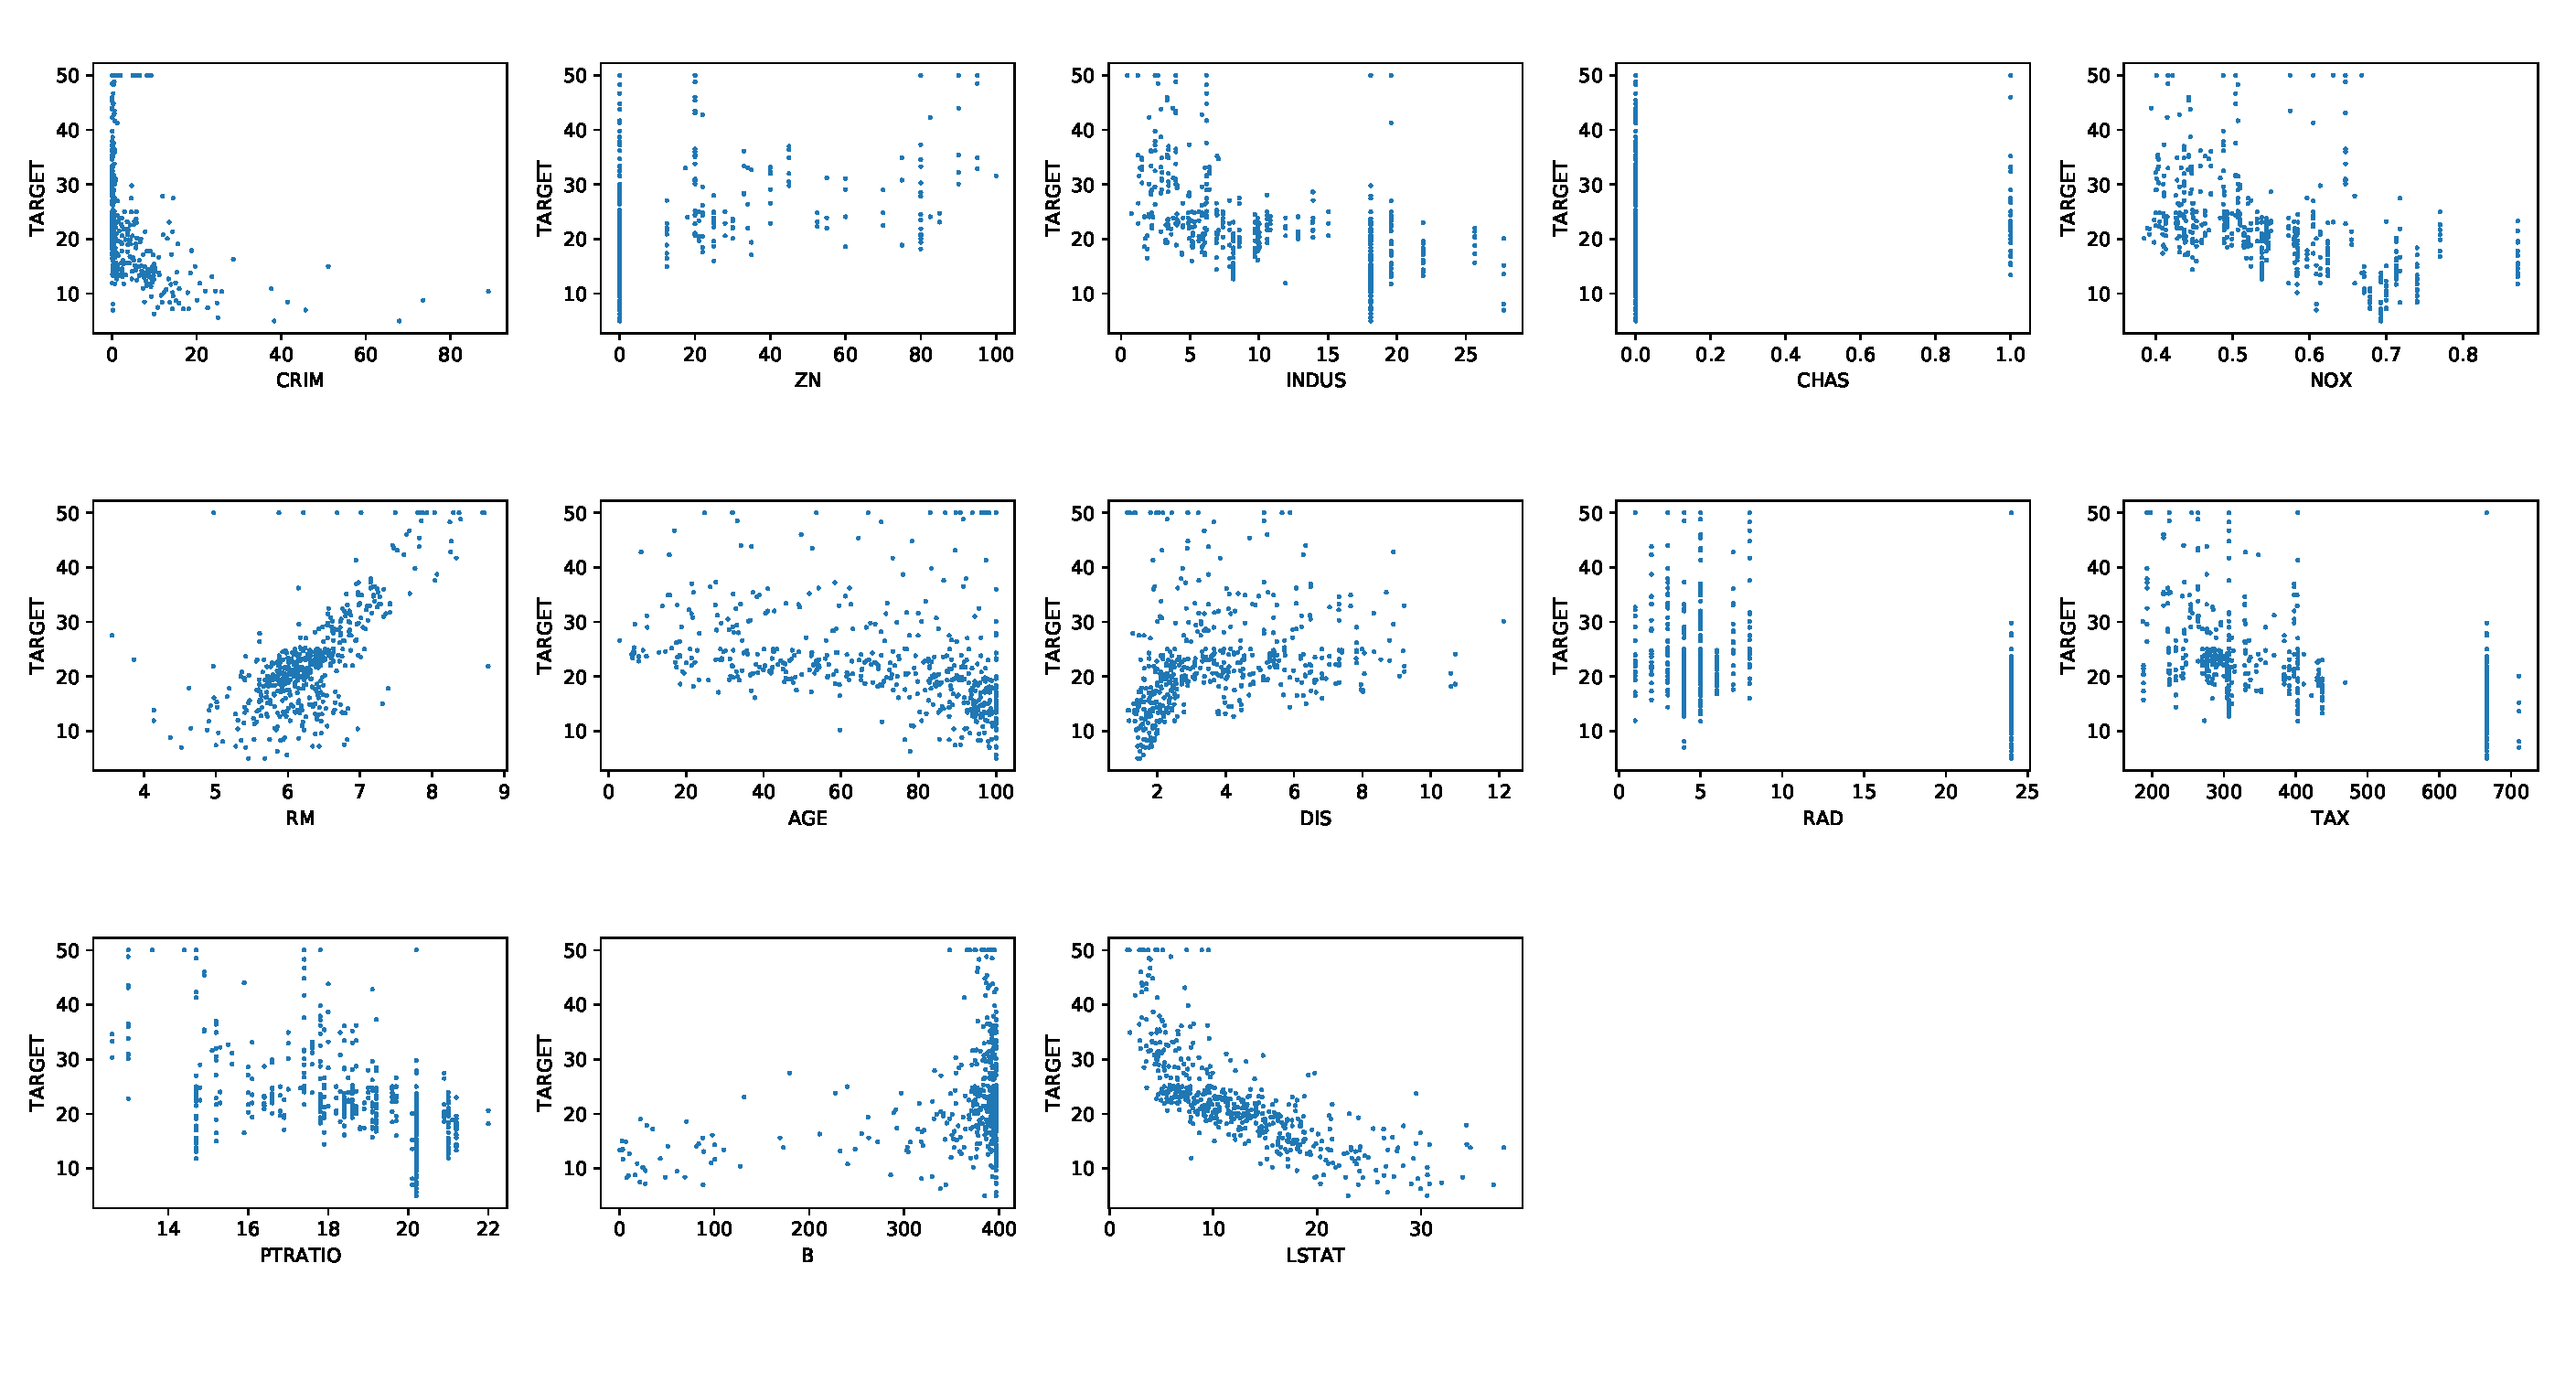
\includegraphics[width = 15cm]{DataDistribution}
\caption{Data points against target for each feature}
\label{fig: Data distribution}
\end{figure}

\subsection{Data division}

To divide training data set and test data set, in Q1, we use function numpy.random.choice() to implement function split\_data(X, y, training\_ratio = 0.2).

\begin{lstlisting}[language = Python]
def split_data(X, y, training_ratio = 0.2):
    test_chosen = np.random.choice(len(X), int(len(X) * training_ratio))
    ......
    return training_set_x, test_set_x, training_set_y, test_set_y
\end{lstlisting}

In the function, we split $X$ and $y$ into $training_set_x$, $test_set_x$, $training_set_y$, $test_set_y$ according to $training_ratio$ for future usage.

\subsection{Linear regression}

To solve linear regression problem and get the weightes $w$, we use numpy.linalg.solve() on the formula:

\begin{equation}
X^\mathrm{T}Xw^*=X^\mathrm{T}y
\end{equation}

\subsection{Feature weights}

After the calculation, we can get the weight on each feature as shown in Table\ref{tab: Feature weights}

\begin{table}[htbp]
\centering
\begin{tabular}{|c|c|c|}
    \hline
    Feature & Weight & Mean\\
    \hline
    CRIM & 41.795688882257188 & 3.5937607114624512\\
    \hline
    ZN & -0.13159561392787489 & 11.363636363636363\\
    \hline
    INDUS & 0.056336470652065491 & 11.136778656126481\\
    \hline
    CHAS & 0.033639549287715828 & 0.069169960474308304\\
    \hline
    NOX & 3.7698365450326135 & 0.55469505928853757\\
    \hline
    RM & -19.35371695539391 & 6.2846343873517787\\
    \hline
    AGE & 3.1091523339672826 & 68.574901185770756\\
    \hline
    DIS & 0.010472276182880488 & 3.7950426877470358\\
    \hline
    RAD & -1.5681353658907364
     & 9.5494071146245059\\
    \hline
    TAX & 0.33065329716511299 & 408.23715415019763\\
    \hline
    PTRATIO & -0.011395113448445227 & 18.455533596837945\\
    \hline
    B & -0.97967928714208496 & 356.67403162055342\\
    \hline
    LSTAT & 0.0096343495439206173 & 12.653063241106722\\
    \hline
    \end{tabular}
\caption{Feature weights}
\label{tab: Feature weights}
\end{table}

Here, we take the feature 'INDUS' (proportion of non-retail business acres per town) as an analysis example. Shown in Table\ref{tab: Feature weights}, we can see feature 'INDUS' has a weight of 0.056336470652065491. As a positive weight, the sign means that is has a positive influence in the target, the housing price. In general ideas, people likes to live in the areas with more shops, which means that house price could be higher. That just fits the result.

\subsection{Model test}
We use $20\%$ of the data as test date to just the fitness of the model. Here are some results of different metics:

\begin{itemize}
    \item MSE: 18.268879264780917
    \item MAE: 3.1172529292203892
    \item R2: 0.75025578036036022
\end{itemize}

These numbers could change due to different training-test dataset division.

\subsection{Feature selection}

To choose the most significan feature, weight of teh featuers are a good metrics. However, due to the different magnitudes of weights, we decide to multiply weight and mean for each feature and use it as the influnce on the target. It is shown as FIgure\ref{tab: Feature influence}.

\begin{table}[htbp]
\centering
\begin{tabular}{|c|c|}
    \hline
    Feature & Inluence\\
    \hline
    CRIM & 150.2037046136\\
    \hline
    ZN & -1.4954047037\\
    \hline
    INDUS & 0.6274068039\\
    \hline
    CHAS & 0.0023268463\\
    \hline
    NOX & 2.0911097059\\
    \hline
    RM & -121.6310351009\\
    \hline
    AGE & 213.2098140733\\
    \hline
    DIS & 0.0397427352\\
    \hline
    RAD & -14.9747630197\\
    \hline
    TAX & 134.9849610451\\
    \hline
    PTRATIO & -0.2103028991\\
    \hline
    B & -349.4261610401\\
    \hline
    LSTAT & 0.1219040341\\
    \hline
    \end{tabular}
\caption{Feature weights}
\label{tab: Feature influence}
\end{table}

From the table, we can see that the feature 'B' has the largest absolute value, which means 'B' predicts the price best.

\section{Q2: Locally reweighted regression}

\subsection{$w^*$ solution proof}

Given $(x^{(1)}, y^{(1)}), \dots, (x^{(N)}, y^{(N)})$ and positive weights $a^{(1)}, \dots, a^{(N)}$, show that the solution to the weighted least square ploblem

\begin{equation}
w^*=\operatorname{argmin}\frac{1}{2}\sum_{i=1}^Na^{(i)}(y^{(i)}-w^\mathrm{T}x^{(i)})^2+\frac{\lambda}{2}\|w\|^2
\end{equation}

is given bu the formula

\begin{equation}
w^*=(X^\mathrm{T}AX+\lambda I)^{-1}X^\mathrm{T}Ay
\end{equation}

where $X$ is the design matrix (defined in class) and $A$ is a diagonal matrix where $A_{ii}=a^{(i)}$

\begin{proof}
    \begin{align*}
        w^*&=\operatorname{argmin}\frac{1}{2}\sum_{i=1}^Na^{(i)}(y^{(i)}-w^\mathrm{T}x^{(i)})^2+\frac{\lambda}{2}\|w\|^2\\
        L(w^*)&=\frac{1}{2}\sum_{i=1}^Na^{(i)}(y^{(i)}-w^\mathrm{T}x^{(i)})^2+\frac{\lambda}{2}\|w\|^2\\
        &=\frac{1}{2}A\|y-Xw\|^2+\frac{\lambda}{2}\|w\|^2\\
        &=\frac{1}{2}(y-Xw)^\mathrm{T}A(y-Xw)+\frac{\lambda}{2}\|w\|^2\\
        &=\frac{1}{2}(y^\mathrm{T}Ay-2w^\mathrm{T}X^\mathrm{T}Ay+w^\mathrm{T}X^\mathrm{T}AXw)+\frac{\lambda}{2}\|w\|^2\\
        \nabla L(w^*)&=\frac{1}{2}(-2X^\mathrm{T}Ay+2X^\mathrm{T}AXw)+\lambda w\\
        &=X^\mathrm{T}AXw+\lambda w-X^\mathrm{T}Ay\\
    \end{align*}
    \qquad Setting this gradient to zero gives\\
    \begin{align*}
        X^\mathrm{T}Ay&=X^\mathrm{T}AXw+\lambda w\\
        w^*&=(X^\mathrm{T}AX+\lambda I)^{-1}X^\mathrm{T}Ay
    \end{align*}
\end{proof}

\subsection{LRLS implementation}

Some essential things in LRLS implemented:

\begin{itemize}
    \item $\|x-x^{(i)}\|^2$ in $a^{(i)}$ calculation: using provided function l2(A,B)
    \item solving $w^*$: using numpy.linalg.solve()
    \item avoiding overflows/underflows: adding $-max_jA_j$in square distance calculation
\end{itemize}

\subsection{K-fold corss-validation}

In this question, we choose $\tau$ from$[10, 1000]$ and proceed cross-validation on different $\tau$value. The variation of loss value is shown in Figure\ref{fig: Tau_loss}.

\begin{figure}[htbp]
\centering
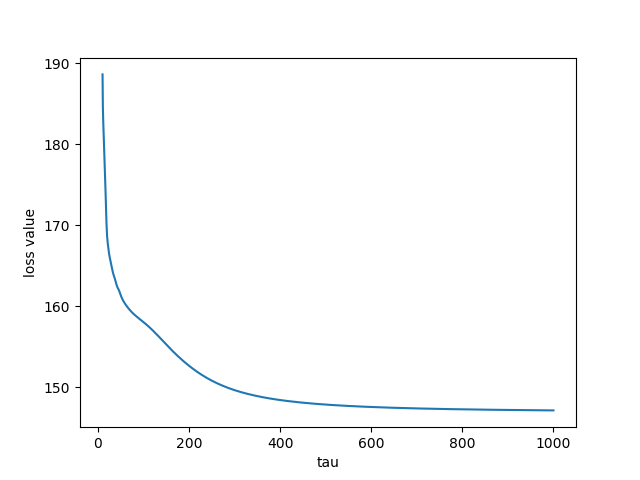
\includegraphics[width = 8cm]{tau-lossvalue}
\caption{Loss value for each $\tau$}
\label{fig: Tau_loss}
\end{figure}

From the figure we can see that, loss value has the following tending:

\begin{itemize}
    \item when$\tau \to 0$, loss value tends towards $+\infty$
    \item when$\tau \to +\infty$, loss value tends tpwards $0$
\end{itemize}

For $\tau$ in$[10, 1000]$, mean value of the loss is 158.987350941, and the minimun value of the loss is 147.119838286.

\bibliographystyle{plain}
\bibliography{bibliography.bib}
\end{document}
